\documentclass{article}

\usepackage{enumerate}
\usepackage{times}
\usepackage{amssymb, amsmath, amsthm}
\usepackage[margin=.5in]{geometry}
\usepackage{graphicx}
\usepackage[linewidth=1pt]{mdframed}

\usepackage{listings}
\usepackage{import}
\usepackage{xifthen}
\usepackage{pdfpages}
\usepackage{transparent}

\newcommand{\incfig}[1]{%
    \def\svgwidth{.8\columnwidth}
    \import{./figures/}{#1.pdf_tex} 
}

\newtheorem{theorem}{Theorem}[section]
\newtheorem{lemma}{Lemma}[section]
\newtheorem*{remark}{Remark}
\theoremstyle{definition}
\newtheorem{definition}{Definition}[section]

\begin{document}

\title{Machine Learning and Data Mining --- Homework 4}
\author{Philip Warton}
\date{\today}
\maketitle
\section{Exercises: Decision Trees and Ensembles}
    \subsection*{Q1}
        \begin{mdframed}
            \begin{enumerate}[a.]
                \item Draw the decision boundaries defined by this tree over the interval $x_1 \in [0, 30]$, $x_2 \in[0, 30]$. Each leaf of
                the tree is labeled with a letter. Write this letter in the corresponding region of input space.
                \item Give another decision tree that is syntactically different (i.e., has a different structure) but defines the
                same decision boundaries.
                \item This demonstrates that the space of decision trees is syntactically redundant. How does this redundancy
                influence learning --- i.e., does it make it easier or harder to find an accurate tree?
            \end{enumerate}
        \end{mdframed}
        \begin{figure}[ht]
            \centering
            \begin{minipage}{.5\textwidth}
                \centering
                \incfig{q1_a}
                \caption{Decision boundary given by tree in Q1}
                \label{fig:}
            \end{minipage}%
            \begin{minipage}{.5\textwidth}
                \centering
                \incfig{q1_b}
                \caption{An equivalent -- but different -- binary decision tree}
                \label{fig:}
            \end{minipage}
        \end{figure}
        \subsubsection*{a.}
        The decision boundary determined by the given tree is illustrated 
        in \fbox{Figure 1}.
        \subsubsection*{b.}
        The equivalent tree that is syntatically different is illustrated in
         \fbox{Figure 2}.
        \subsubsection*{c.}
            The redundancy phenomenon makes it much easier for learning, 
            since it means that there are many different ways to get to the 
            correct solution, so we will still have logical equivalence 
            under different starting conditions, making learning not have 
            to be as strict/stringent to find the exact unique solution 
            desired.
    \subsection*{Q2}
        \begin{mdframed}
            Consider the following training set and learn a decision 
            tree to predict Y. Use information gain to select attributes 
            for splits.
            \begin{center}
                \begin{tabular}{lll|l}
                    A & B & C & Y \\
                    \hline
                    0 & 1 & 1 & 0 \\
                    1 & 1 & 1 & 0 \\
                    0 & 0 & 0 & 0 \\
                    1 & 1 & 0 & 1 \\
                    0 & 1 & 0 & 1 \\
                    1 & 0 & 1 & 1
                \end{tabular}
            \end{center}
            For each candidate split include the information gain in your 
            report. Also include the final tree and your training accuracy.
        \end{mdframed}
        % TODO Complete this section 
    \subsection*{Q3}
        \begin{mdframed}
            \begin{enumerate}[a.]
                \item Apply bagging by uniformly sampling train datapoints 
                    with replacement to train each ensemble member.
                \item The sklearn API for the DecisionTreeClassifier 
                    provides many options to modify how decision trees 
                    are learned, including some of the techniques we 
                    discussed to increase randomness. When set less than 
                    the number of features in the dataset, the 
                    \begin{verbatim}max_features\end{verbatim}
                    argument will cause each split to only consider a 
                    random subset of the features. Modify line 44 to 
                    include this option at a value you decide.
            \end{enumerate}
        \end{mdframed}
        \subsubsection*{a.}
            We apply bagging to the decision try ensemble members by 
            modifying lines 39-42 as follows:
            \begin{lstlisting}[language=python]
  n = len(X_train)
  rand_idx = np.random.choice(n, n, replace=True)
  X_data = X_train[rand_idx,:]
  y_data = y_train[rand_idx]
            \end{lstlisting}
            \begin{figure}[htpb]
                \centering
                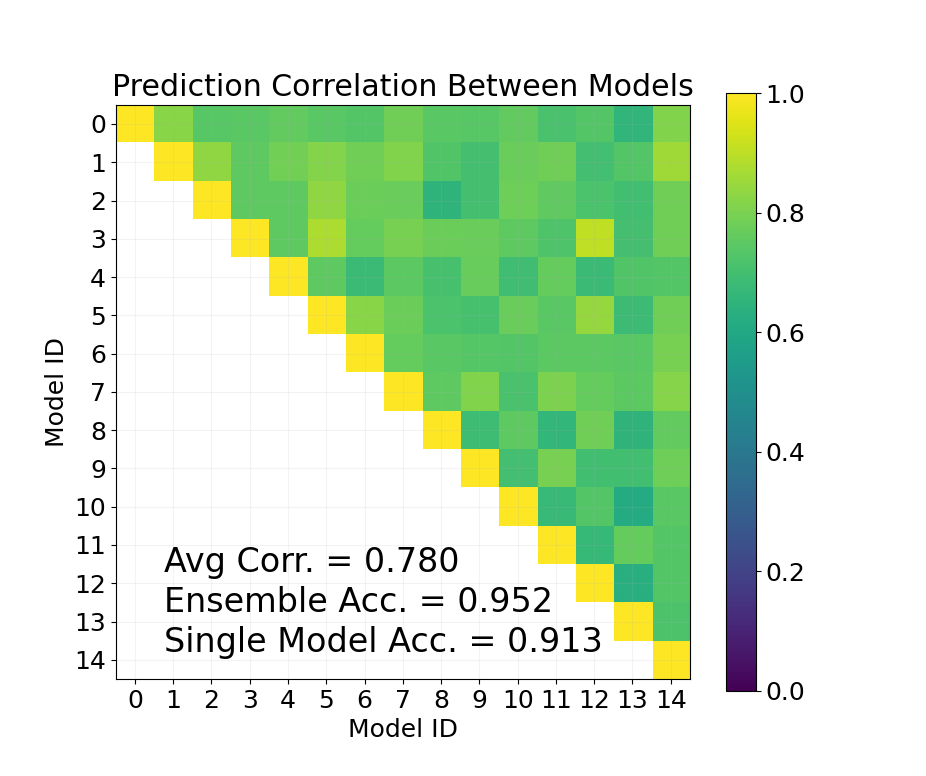
\includegraphics[width=0.4\textwidth]{figures/q3_a.png}
                \caption{Prediction correlation between models with ensemble
                -wise bagging}
                \label{fig:}
            \end{figure}
        \subsubsection*{b.}
            In order to change the maximum number of features learned, we 
            modify line 44 to be 
            \begin{lstlisting}[language=python]
clf = tree.DecisionTreeClassifier(criterion="entropy", max_features="auto")
            \end{lstlisting}
            What this does is it changes the maximum number of features to 
            be about $\sqrt{n}$ ($n$ being the number of features total),
            which results in a similar kind of correlation graph as in 
            \fbox{Part a}.
            \begin{figure}[htpb]
                \centering
                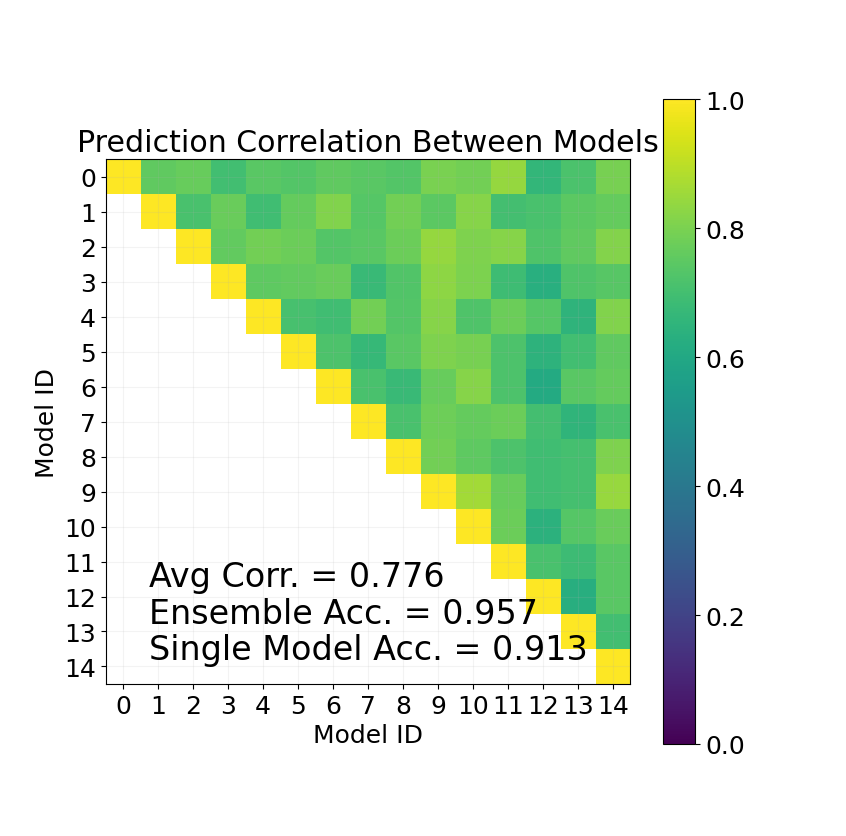
\includegraphics[width=0.4\textwidth]{figures/q3_b.png}
                \caption{Prediction correlation between models with 
                    $\sqrt n$ max features}
                \label{fig:}
            \end{figure}
\section{Implementation: k-Means Clustering}
    \subsection*{Q4}
       \begin{mdframed}
           The provided skeleton code file kmeans.py implements the main 
           k-means function but includes stubs for the following functions: 
           initializeCentroids, computeAssignments, updateCentroids, and 
           calculateSSE. Implement these functions to finish the 
           implementation. The code provides input/output specifications
       \end{mdframed} 
       \subsubsection*{a.}
       \begin{lstlisting}[language=python]
def initalizeCentroids(dataset, k):

  # Choose k distinct random indices and set our centroids to their
  # corresponding points
  rand_idx = np.random.choice(len(dataset), size=k, replace=False)
  centroids = dataset[rand_idx,:]
  return centroids
       \end{lstlisting}
       \subsubsection*{b.}
       \begin{lstlisting}[language=python]
def computeAssignments(dataset, centroids):

  # Set length variable for readability
  n = len(dataset)

  # Initialize vector for assignment idx
  assignments = np.zeros((n,1))

  # Loop over each point in dataset
  for i in range(0,n):
    x_i = dataset[i]

    # Take difference of x_i and each centroid
    # and take their norms
    norms = np.linalg.norm(centroids - x_i, axis=1)

    # Get idx of closest centroid and set assign to point
    assignments[i] = np.argpartition(norms, kth=0)[0:1]

  return assignments
       \end{lstlisting}
       \subsubsection*{c.}
       \begin{lstlisting}[language=python]
def updateCentroids(dataset, centroids, assignments):
  counts = []
  for j in range(0, len(centroids)):

    # To count number of x_i assigned to c_j
    num_assigned = 0

    # To sum them
    sum_assigned = np.zeros(dataset[0].shape)

    # Here we preform the sum
    for i in range(0, len(dataset)):

      # If point x_i is assigned to c_j
      if j == assignments[i]:

        # Iterate count and add it to sum
        num_assigned += 1
        sum_assigned += dataset[i]

    counts.append(num_assigned)

    # Avg of assigned points becomes new centroid
    centroids[j] = sum_assigned / num_assigned

  return centroids, counts
       \end{lstlisting}
       \subsubsection*{d.}
       \begin{lstlisting}[language=python]
def calculateSSE(dataset, centroids, assignments):
  sse = 0
  for i in range(0, len(assignments)):
    error = np.linalg.norm(dataset[i] - centroids[int(assignments[i])])
    sq_error = error ** 2
    sse += sq_error
  return sse
       \end{lstlisting}
    \subsection*{Q5}
        In order to see the random distribution as desired, we modify our 
        code to be
        \begin{lstlisting}[language=python]
for i in range(0, 50):
  SSE = kMeansClustering(X, k=k, max_iters=max_iters, visualization=False)[2]  
  SSE_rand.append(SSE)
        \end{lstlisting}
        This ultimately gives us the histogram for the distribution
        of random SSE's given by \fbox{Figure 5}
        \begin{figure}[htpb]
            \centering
            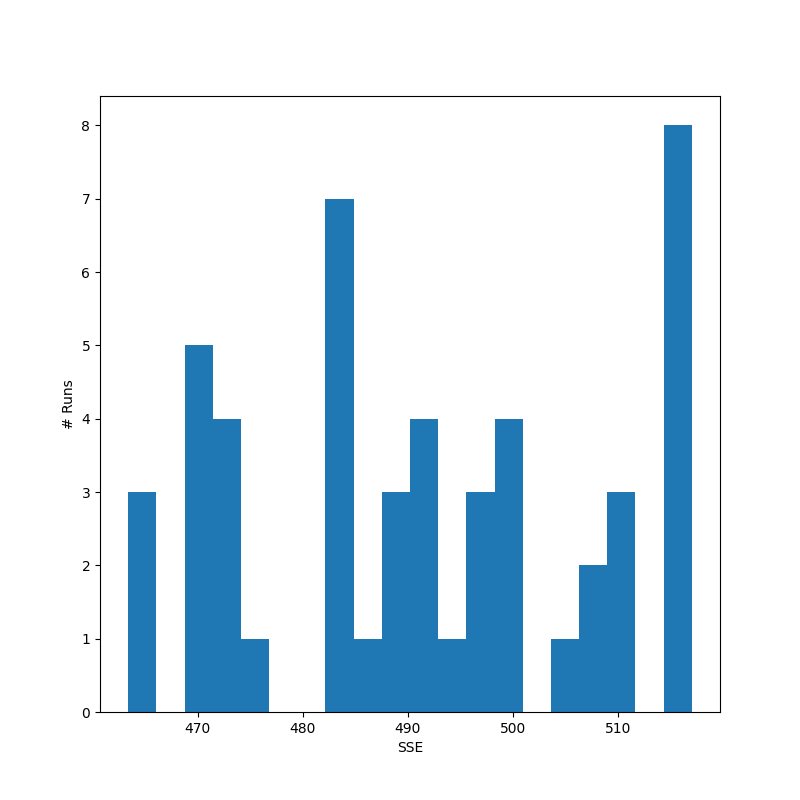
\includegraphics[width=0.4\textwidth]{figures/q5.png}
            \caption{SSE histogram on 50 random trials}
            \label{fig:}
        \end{figure}
        What we see looks like what could possibly be a uniform distribution
        maybe with a lot of noise. Regardless, it is clear that our SSE can 
        vary randomly quite a bit, and perhaps it would be good to ensure 
        that we are running the algorithm several times and choosing the 
        best model, when we use this on real life data.
    \subsection*{Q6}
        \begin{mdframed}
            One important question in k-means is how to choose k. In prior 
            exercises, we’ve chosen hyperparmeters like this based on 
            performance on some valdiation set; however, k-means is an 
            unsupervised method so we don’t have any labels to compute 
            error. One idea would be to pick k such that the sum-of-
            squared-errors is minimized; however, this ends up being a bad 
            idea – let’s see why. Finish the following code on the 
            toyProblem function to run k-means with $k = 1,2,\cdots,150$ 
            on the toy dataset and plot the final SSE achieved for each 
            clustering.
        \end{mdframed}
        To run this experiment, we implement the following code
        \begin{lstlisting}[language=python]
for i in range(0,150):
  SSE = kMeansClustering(X, k=i+1, max_iters=20, visualize=False)[2][-1]
  SSE_vs_k.append(SSE)
        \end{lstlisting}
        Then, we see an exponentially decaying relationship between SSE and 
        $k$ \fbox{Figure 6}. This means that if we minimize SSE we will always end up with 
        $k = n$, which is not at all useful.
        \begin{figure}[htpb]
            \centering
            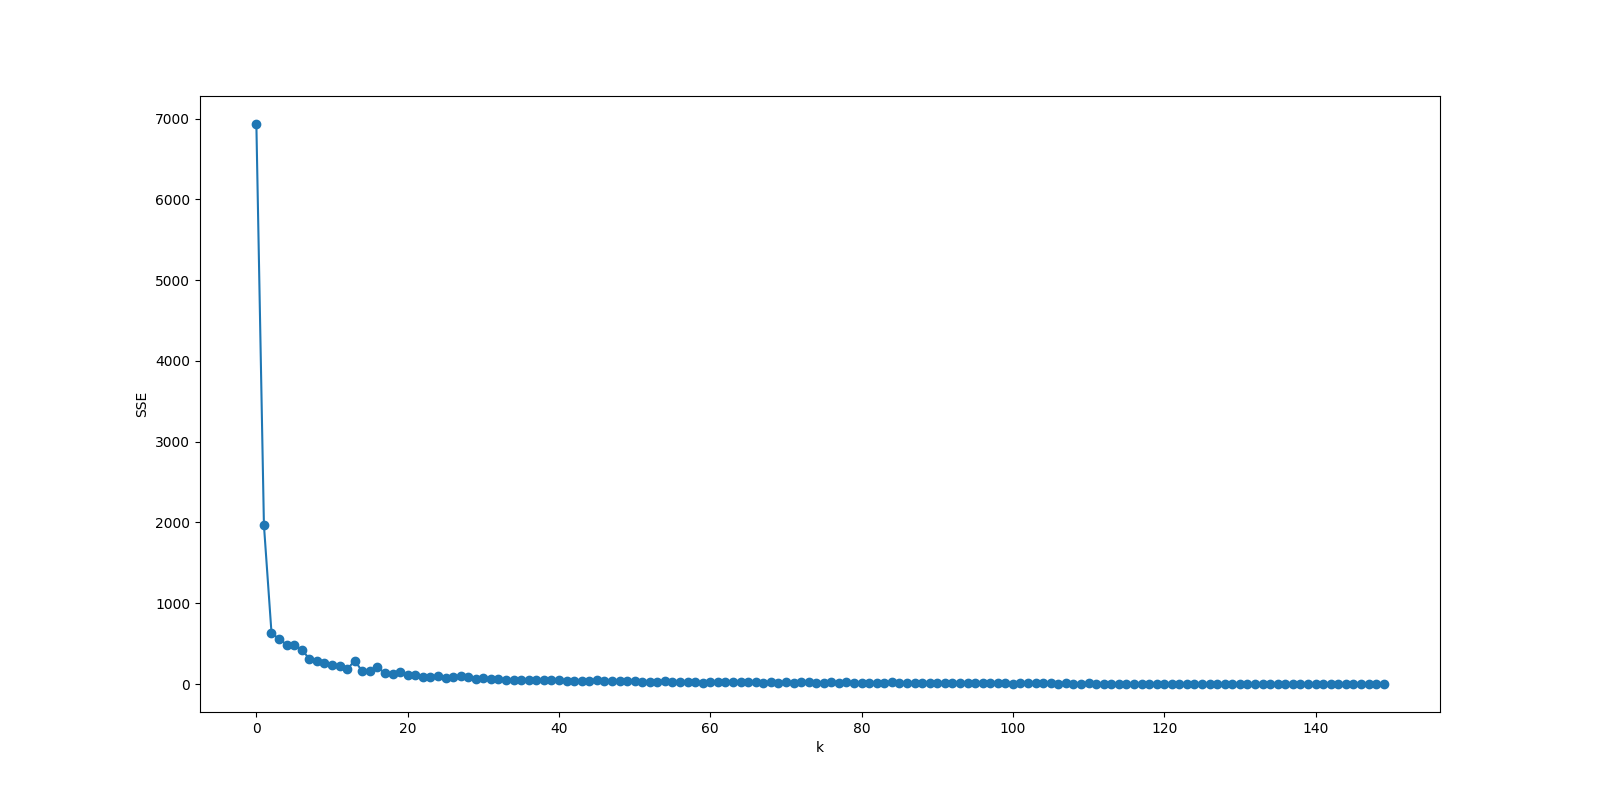
\includegraphics[width=0.8\textwidth]{figures/q6.png}
            \caption{SSE vs $k$ for the toy problem}
            \label{fig:}
        \end{figure}
    \subsection*{Q6}
        \begin{mdframed}
            Inside kmeans.py, the imageProblem function runs your k-means 
            algorithm on this set of images and features and then 
            visualizes the resulting clusters by showing up to 50 samples. 
            By default, the code runs with k = 10 for this dataset. Answer:
            \begin{enumerate}[a.]
                \item From the images displayed, describe what types of 
                    images are in the dataset. Does the default parameter 
                    of k = 10 seem to be too high, too low, or fine as it is?
                \item Adjust k until you are happy with the clusters you 
                    observe. Include the samples from your clusterings.
                \item Compare the SSE for your chosen k against the SSE 
                    from k = 10. Is SSE a good indicator of clustering 
                    quality?
            \end{enumerate}
        \end{mdframed}
        \subsubsection*{a.}
            By the looks of it, there are vaguely 3 different kinds of 
            images. There are images of skyscrapers, empty roads, and lush 
            greenery. So, I would guess that $k=10$ is too high because 
            there are multiple clusters that seem very similar in character.
        \subsubsection*{b.}
            I started by adjusting $k$ to 3, and as it turns out this was 
            the best one that I could ultimately come up with. In 
            \fbox{Figures 7-9}, a sample from each cluster is displayed.
        \subsection*{c.}
            For the SSE, we have
            \begin{align*}
                k &= 3 \Rightarrow &SSE &= 2963.57 \\
                k &= 10 \Rightarrow &SSE &= 2375.55
            \end{align*}
            As we can see, the SSE is much smaller for $k=10$ than for
            $k=3$. However, similar to our answer for Q6 we conclude 
            that SSE is not a reliable metric to minimize, since more 
            clusters are always favored. So, we say that no, SSE is not 
            a good indicator of cluster quality.
    \subsection*{Q8}
        Here we have our figures of the samples of our clusters, 
        and the associated purities of each, given in \fbox{Figures 7-9}.
        \begin{figure}
            \begin{subfigure}{\textwidth}
              \begin{minipage}[c]{0.67\textwidth}
                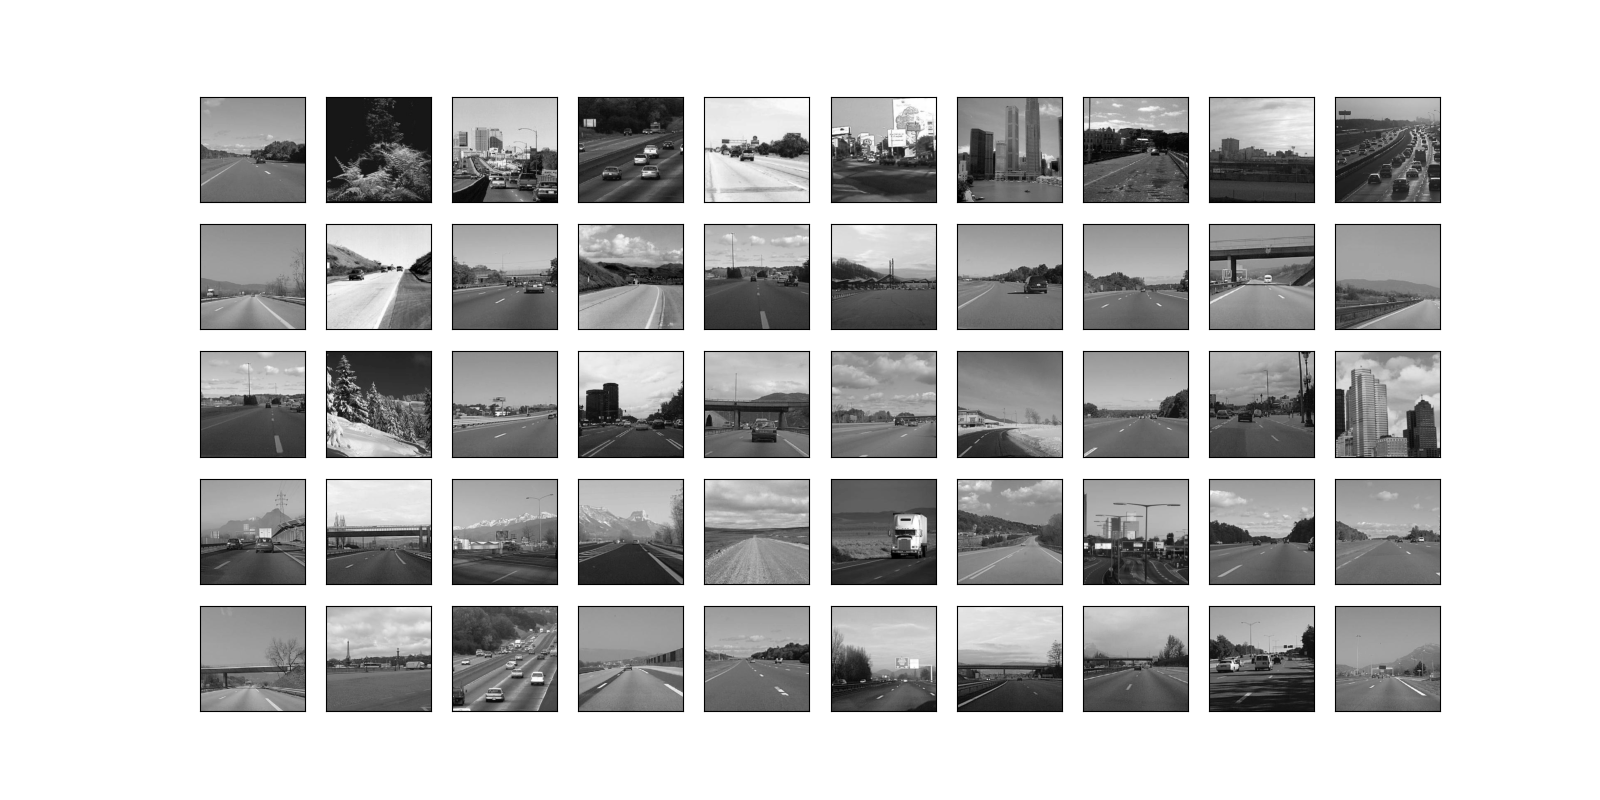
\includegraphics[width=\textwidth]{figures/q7_b_1.png}
              \end{minipage}\hfill
              \begin{minipage}[c]{0.3\textwidth}
                \caption{
                    Cluster 1 --- Roads \\
                    numViolations = 4 \\
                    purity = 92\%
                } \label{fig:}
              \end{minipage}
            \end{subfigure}
            \begin{subfigure}{\textwidth}
              \begin{minipage}[c]{0.67\textwidth}
                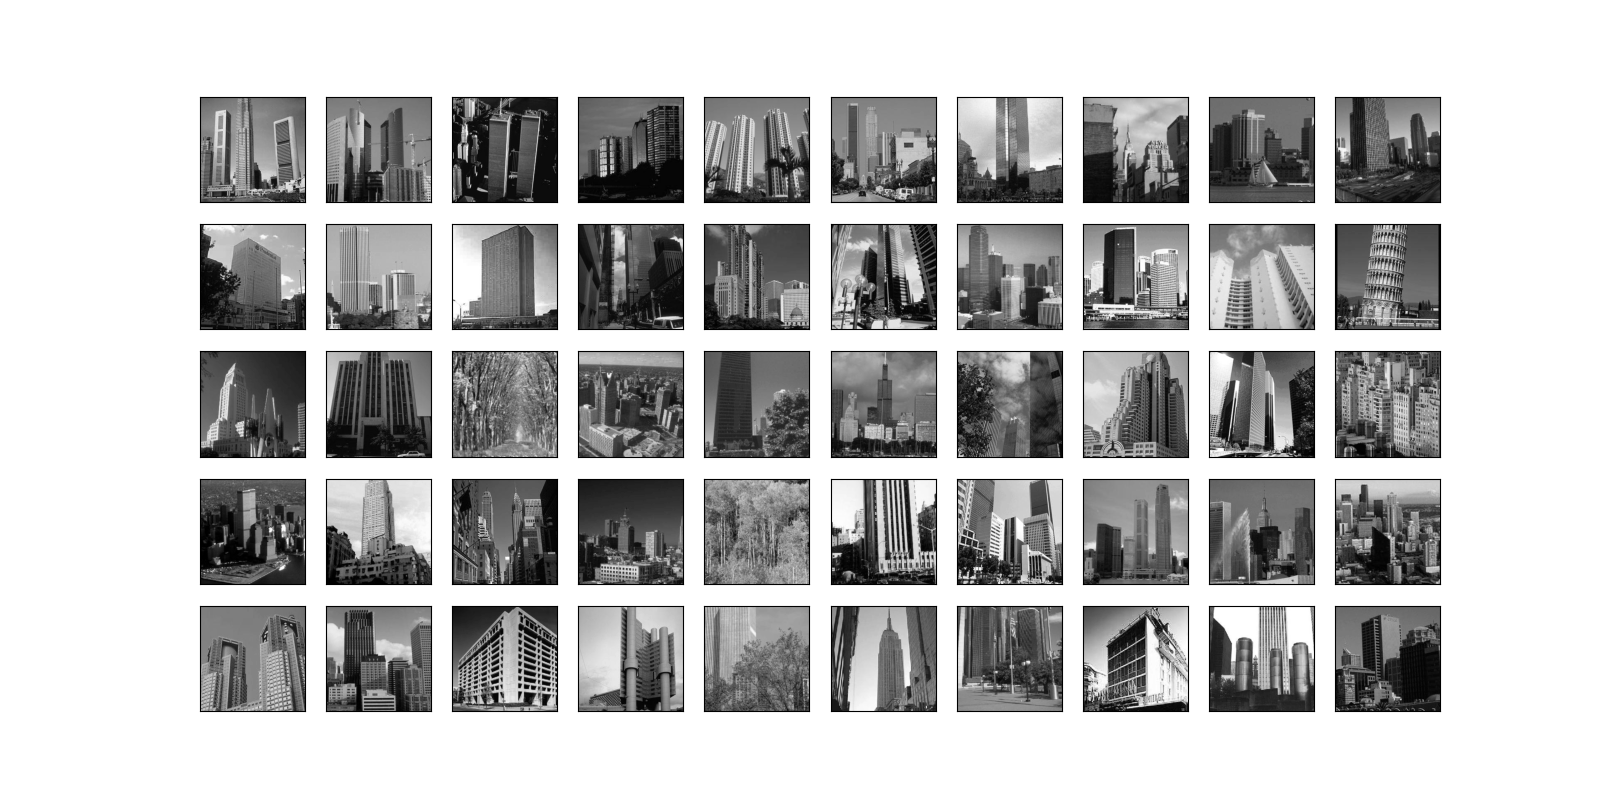
\includegraphics[width=\textwidth]{figures/q7_b_2.png}
              \end{minipage}\hfill
              \begin{minipage}[c]{0.3\textwidth}
                \caption{
                    Cluster 2 --- Buildings \\
                    numViolations = 2 \\
                    purity = 96\%
                } \label{fig:}
              \end{minipage}
            \end{subfigure}
            \begin{subfigure}{\textwidth}
              \begin{minipage}[c]{0.67\textwidth}
                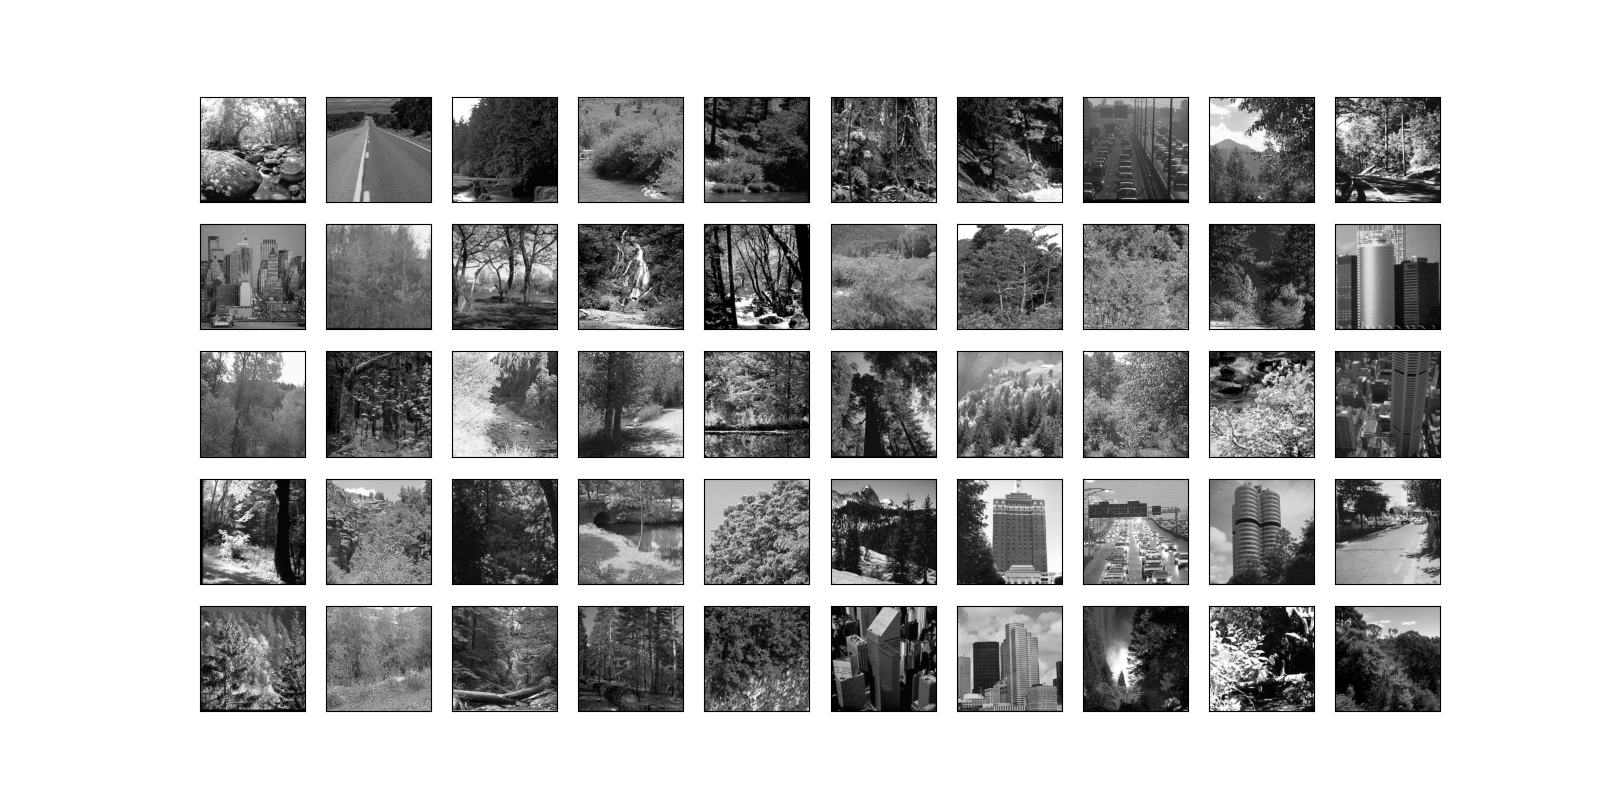
\includegraphics[width=\textwidth]{figures/q7_b_3.png}
              \end{minipage}\hfill
              \begin{minipage}[c]{0.3\textwidth}
                \caption{
                    Cluster 3 --- Greenery \\
                    numViolations = 10 \\
                    purity = 80\%
                } \label{fig:}
              \end{minipage}
            \end{subfigure}
        \end{figure}
\section{Debriefing}
    \begin{enumerate}
        \item 12 hours total on this assignment
        \item Assigment was moderate difficulty -- Q2 was tough
        \item Worked mostly alone on this, recieved some advice on Q2
        \item I understand the material about 50\%. I don't feel good about 
            the decision tree stuff, but $k$-means I feel is quite easy to 
            have a grasp of.
        \item No other comments
    \end{enumerate}
\end{document}
